\documentclass{article} 
\usepackage{amsmath} 
\usepackage{graphicx} 
\usepackage[top=1in, bottom=1in, left=.65in, right=.65in]{geometry} 
\usepackage{fancyhdr} 
\usepackage{multicol}
\usepackage{capt-of}
\usepackage[font=footnotesize,labelfont=bf]{caption}
\usepackage{siunitx}
\usepackage{tabularx}
\usepackage[parfill]{parskip}
%standard 2 column lab report template.

%scale = .22 for in/out plots
%scale = .4 for reg plots

%%%define figure environment, headers. remove section numbering.
\newenvironment{2colfig}{
  \par\medskip\noindent\minipage{\linewidth}
} {
  \endminipage\par\medskip
}

\newcommand{\labhead}[1]{
  \vspace{1em}
  {\bf #1}$_{\,}$
  \hline
  \vspace{1em}
}

\makeatletter
\newlength \figwidth
\if@twocolumn
  \setlength \figwidth {0.9\columnwidth}
\else
  \setlength \figwidth {0.5\textwidth}
\fi
\makeatother%

\setcounter{secnumdepth}{0}

\begin{document}
\lhead{PH 481 - Lab 2.}
\chead{Rene Zeto} 
\rhead{\thepage} 
\pagestyle{fancy} 
\fancyfoot[c]{} 
\setlength{\parindent}{0pt}

\begin{multicols*}{2}
\labhead{Introduction.}
In this lab, we explore different properties of light incidence on glass surfaces. We will first measure the
transmission and reflectivity of a laser incident on a glass mirror and glass coverslip. We will then compare this data
to the theoretical Fresnel equations, and check for consistent behavior. Then, we will measure the refractive index of a
plastic slab, by shooting a laser at it, and measuring the deflection angle. Finally, we will send a beam through a
Fresnel Zone Plate, and calculate the radius of the first ring in the diffraction pattern by looking for peak intensity
locations on the optical axis.

\labhead{Theory.}
We must again make use of Snell's law, particularly for calculating the Brewster angle and refractive index of the plastic slab.
\begin{equation}
  \label{equation:snells}
  n_1 \sin{\theta_1} = n_2 \sin{\theta_2}.
\end{equation}
Additionally, we must use the Fresnel equations. They are, for S-polarized light:
\begin{equation}
  \label{equation:rs}
  R_s = \left| \frac{n_1 \cos\theta_i - n2\sqrt{1-\left(\frac{n_1}{n_2}\sin\theta_i\right)^2}}{n_1 \cos\theta_i+n_2\sqrt{1-\left(\frac{n_1}{n_2}\sin\theta_i\right)^2}}\right|^2,
\end{equation}
which is the reflectivity, and 
\begin{equation}
  \label{equation:ts}
  T_s = 1 - R_s,
\end{equation}
which is the transmission. For P-polarized light:
\begin{equation}
  \label{equation:rp}
  R_p = \left| \frac{n_1 \sqrt{1-\left(\frac{n_1}{n_2}\sin\theta_i\right)^2} - n_2 \cos\theta_i}{n_1\sqrt{1-\left(\frac{n_1}{n_2}\sin\theta_i\right)^2}+n_2\cos\theta_i}\right|^2,
\end{equation}
and
\begin{equation}
  \label{equation:tp}
  T_p = 1 - R_p.
\end{equation}
For the last part of the lab, we can calculate the diffraction ring radius using the optical axis distance using the following relationship:
\begin{equation}
  \label{equation:frz}
  f_1 = \frac{R_1^2}{\lambda}.
\end{equation}
\labhead{Experiment.}
We did four main experiments for this lab. 


{\bf 1. Reflection from glass.} The goal of the first experiment was to determine the Brewster angle and reflectance of
a glass coverslip. This was done for both S and P polarized light. 

To obtain polarized light for use in the experiment, we powered a regular HeNe laser, and sent the beam along an optical
track, through a linear polarizer. The linear polarizer was rotatable, so we could control which polarization of the
beam was passing through the polarizer. A diagram of the setup is presented in Figure~\ref{fig:exp1}.

\begin{2colfig}
  \center
  \includegraphics[scale=.2]{exp1}
  \captionof{figure}{Optical axis setup for measuring the reflectivity of the glass mirror, mirror 3.}\label{fig:exp1}
\end{2colfig}

The beam is then directed at a mirror (mirror 3) which is mounted on a rotating stage. The mirror then reflects the beam
towards a movable photodetector, with which we can measure the relative intensity of the beam. To measure the
reflectance, we would adjust the angle between the beam connecting mirror 3 and the photodetector, and the beam
connecting mirror 3 and mirror 2, and then we would measure the resulting change in beam intensity using the
photodetector.

{\bf 2. Transmission through glass.} The aim of the second experiment was to measure the tramsmittance of a glass
coverslip. This was done for both S and P polarized light. We used much of the same setup for this experiment as we did
in the previous experiment, but replaced mirror 3 with the glass slide mount. The glass slide mount was sitting on top
of the same rotational stage as mirror 3 was. This time, the photodetector was mounted on the optical track itself, as
is shown in Figure~\ref{fig:exp2}.

\begin{2colfig}
  \center
  \includegraphics[scale=.2]{exp2}
  \captionof{figure}{Optical axis setup for the reflectivity experiment. Similar to Figure~\ref{fig:exp1}, but the
    photodetector has been placed on the optical axis, behind the glass cover slip.}\label{fig:exp2}
\end{2colfig}

We again varied the angle of the stage, and made measurements of the corresponding relative intensity of the transmitted
beam. 

{\bf 3. Refraction.} In this experiment, we used the rotational mount and laser to measure the refractive index $n_2$ of a
thick plastic slab. 

\begin{gather}
  d'\sin(\theta_1 - \theta_2) = L \\
  d'\sin\left(\theta_1 - \sin^{-1}\left(\frac{n_1}{n_2}\sin\theta_1\right)\right) = L \\
  \frac{n_1\sin\theta_1}{\sin\left(\theta_1 - \sin^{-1}\left(\frac{L}{d'}\right)\right)} = n_2
\end{gather}

where $d' = \frac{d}{\cos{\theta_2}}$. 

\begin{2colfig}
  \center
  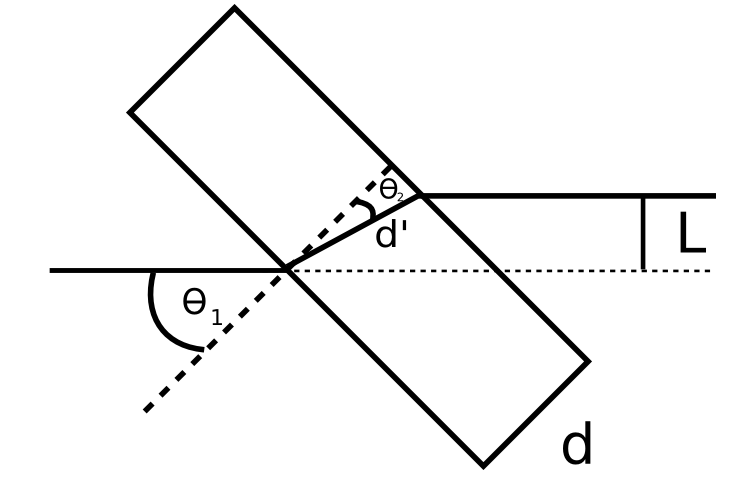
\includegraphics[scale=.2]{mathdrawing}
  \captionof{figure}{Diagram of the geometry of the beam passing through the plastic slab. We measured the beam
    deflection, $L$, the slab thickness, $d$, and the incident angle, $\theta_i$.}\label{fig:mathdrawing}
\end{2colfig}

This formula allows us to calculate $n_2$ based on knowing the deflection distance, the thickness of the slab, and the
angle of incidence. The angle of incidence was controlled by mounting the plastic slab onto the rotational stage. The
deflection distance and slab thickness were measured directly. See Figure~\ref{fig:mathdrawing} for details.

{\bf 4. Fresnel Zone Plate.}
We constructed a beam expander on the optical track (as shown in Figure~\ref{fig:exp4}) using lenses with focal lengths
\SI{25.4}{\milli\meter} and \SI{200}{\milli\meter}, respectively. The expanded and collimated beam then passed through a
Fresnel Zone Plate, creating a diffraction pattern with peak intensities at certain lengths.

\begin{2colfig}
  \center
  \includegraphics[scale=.2]{exp4}
  \captionof{figure}{Beam preparation for passing through Fresnel Zone plate.}\label{fig:exp4}
\end{2colfig}

We placed an index card directly in the beam path, and followed the beam to the wall, noting distances that appeared to
peak intensity spots in the center of the beam. We used this information to compute $R_1$, the outer radius of the first
ring in the diffraction pattern.

\labhead{Results.}
{\bf 1. Reflection from glass.} Plotted in Figures~\ref{fig:data1} and~\ref{fig:data2} are the measured reflectivities and theoretical
reflectivities for the first experiment. The voltage measurements from the photodetector have been normalized (1.0 as
the maximum intensity), and scaled by a factor of $(n_1 - n_2)/(n_1 + n_2)$ for comparison with the corresponding
Fresnel equations.
\begin{2colfig}
  \center
  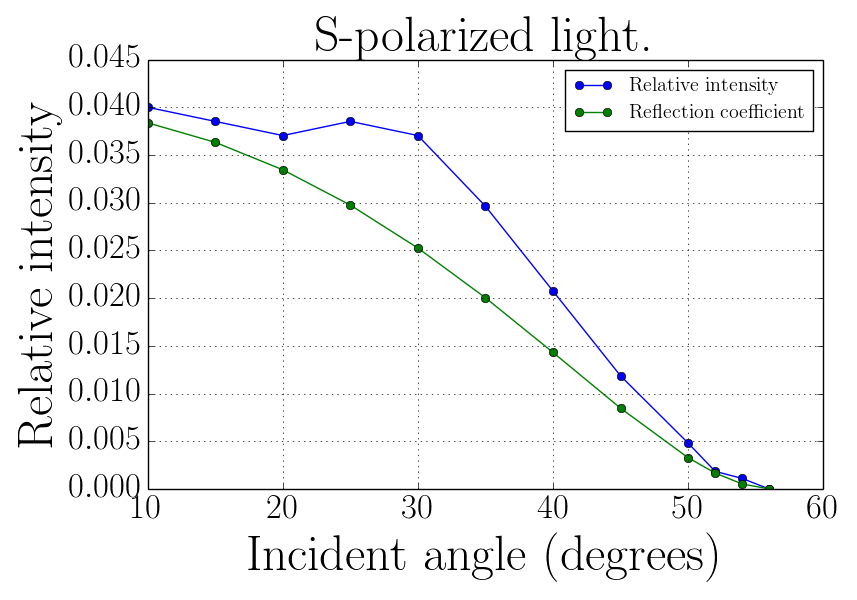
\includegraphics[scale=.4]{data1}
  \captionof{figure}{Reflectivity, both theoretical (green) and measured (blue). P-polarized light.}\label{fig:data1}
\end{2colfig}

\begin{2colfig}
  \center
  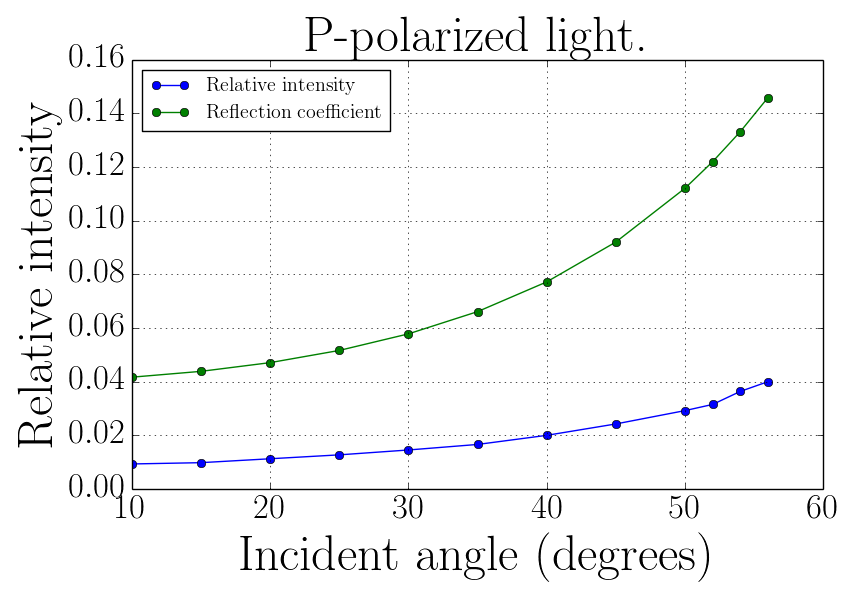
\includegraphics[scale=.4]{data2}
  \captionof{figure}{Reflectivity, both theoretical (green) and measured (blue). S-polarized light.}\label{fig:data2}
\end{2colfig}

{\bf 2. Transmission through glass.} Plotted in Figures~\ref{fig:data3} and~\ref{fig:data4} are the measured
transmissions and theoretical transmissions for the second experiment. The voltage measurements have again been
normalized as they were in first two plots, except they are now scaled by $1 - (n_1 - n_2)/(n_1 + n_2)$ 
\begin{2colfig}
  \center
  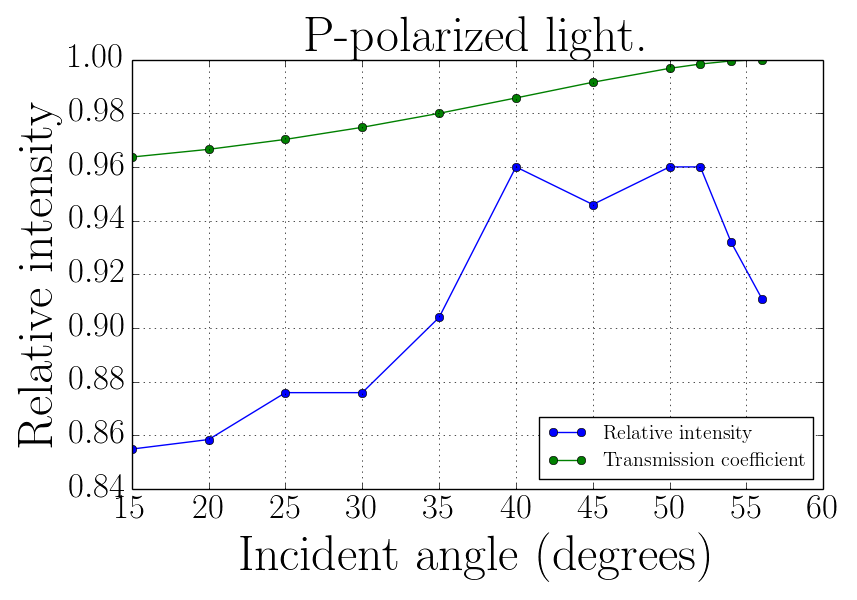
\includegraphics[scale=.4]{data3}
  \captionof{figure}{Transmission, both theoretical (green) and measured (blue). P-polarized light.}\label{fig:data3}
\end{2colfig}

\begin{2colfig}
  \center
  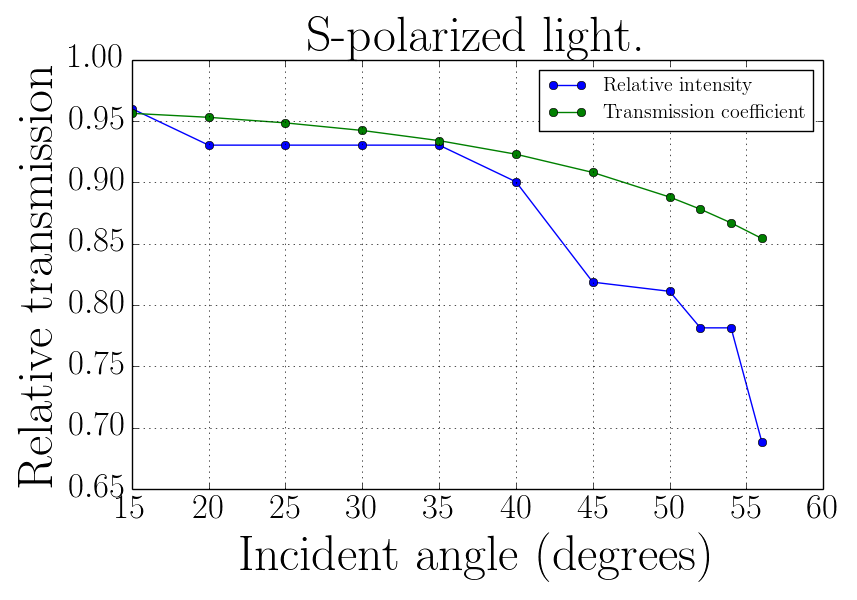
\includegraphics[scale=.4]{data4}
  \captionof{figure}{Transmission, both theoretical (green) and measured (blue). S-polarized light.}\label{fig:data4}
\end{2colfig}

{\bf 3. Refraction.} We measured the thickness of the slab $d$ to be \SI{1.7}{\centi\meter}. With the slab inserted, the
beam was deflected by \SI{1.3}{\centi\meter}. Using Equation 8, the refractive index $n_2$ of the plastic slab is 1.10.

{\bf 4. Fresnel Zone Plate.}  The peak intensity points on the optical axis are listed in Table~\ref{table:table1}. 

\begin{2colfig} 
  \center
  \begin{tabular}{|c|c|c|} \hline
    Intensity peak & Distance\\ \hline
    1 & \SI{49}{\centi\meter} \\ \hline
    2 & \SI{175}{\centi\meter} \\ \hline
  \end{tabular}
  \captionof{table}{Peak intensity locations along optical axis. Distances measured from Fresnel Zone Plate.}\label{table:table1}
\end{2colfig}

Using Equation~\ref{equation:frz}, we calculate the first ring's radius to be \SI{1.05}{\milli\meter}.

\labhead{Uncertainty.}  
One source of uncertainty in this lab was in the second experiment, the measurement of transmission through the glass
cover slip. We noticed that the cover slip caused a lot of unwanted reflection when the beam was passing through
it. Since some of this reflection would reflect off both surfaces and transmit through to the photodetector, this could
have interfered with the intensity measurements we made.

In the third experiment, there was significant uncertainty in measurement of the deflection distance caused by the
plastic slab. We were just marking points on cardboard, and it could have been a little off. The experiment was also
very sensetive to the angle of incidence of the beam, since we chose such a large angle. 

In last experiment, our method for measuring the peak intensity distances had some inherent uncertainty to it. We used a
meterstick for measuring the on axis distance to the peak intensity spot, and the spot itself was sort of difficult to
locate. We minimized this as best we could.

\labhead{Discussion.}  
Although there are some scaling issues, the plots show good agreement with their respective
Fresnel equations. The measured reflectivity and transmittance were relative measurements anyway. We saw decreasing
transmission and reflection of S-polarized light as we approached the Brewster angle for both the coverslip and the
mirror, and increasing transmission and reflection of P-polarized light.

The index of refraction of the plastic slab seems a little low, but it is within an acceptable range, and our imprecise
measurements probably made it a little off. 

Using the Fresnel Zone Plate, we were able to calculate a radius of the first ring in the resulting diffraction pattern
that seemed very reasonable with what we observed in the lab (\SI{1.05}{\milli\meter}). 

\labhead{Conclusion.}
In this lab, we gathered data to plot the transmission and reflection curves of light incident upon a surface. We
plotted these along with the corresponding Fresnel equations to compare theory vs. experiment, and saw good
agreement. We then used a similar technique to calculate the index of refraction of a different material, and obtained a
reasonable result. Finally, we calculated the radius of the first ring in the diffraction pattern caused by sending
light through a Fresnel Zone Plate. 
\end{multicols*}
\end{document}
%% \begin{2colfig}
%%   \center
%%   \includegraphics[scale=.2]{exp3_a}
%%   \captionof{figure}{a simple experiment}\label{fig:exp3_a}
%% \end{2colfig}
%% \begin{2colfig}
%%   \center
%%   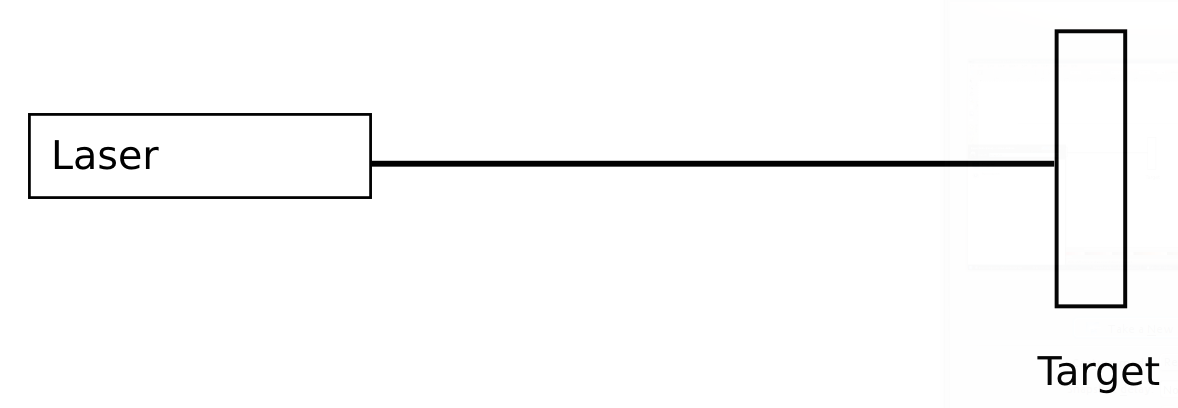
\includegraphics[scale=.2]{exp3_b}
%%   \captionof{figure}{a simple experiment}\label{fig:exp3_b}
%% \end{2colfig}
